\documentclass[12pt]{article}
\usepackage{graphicx}
\usepackage{amsfonts}

%\usepackage{stmaryrd}
\providecommand{\keywords}[1]{\textbf{\textit{KeyWords:}} #1}


\title{\textbf{Practical Fully Secure Three-Party Computation via Sub-linear Distributed Zero-Knowledge Proofs} \break\break Supervisor:\break Niv Gilboa \break}
\author{  Vitali Lopushenko\\
	\texttt{317104347}
	\and
	Osher Saragani\\
	\texttt{315348706}\
	\date{31.8.20}
	}

\begin{document}
\begin{figure}
	\begin{minipage}[c]{0.6\linewidth}
		
\includegraphics[width=\linewidth]{"../Figures/BGU-logo.png"}
	\end{minipage}
	\hfill
	\begin{minipage}[c]{0.3\linewidth}
		
\includegraphics[width=\linewidth]{"../Figures/cse_logo.png"}
	\end{minipage}%
\end{figure}

\maketitle
\pagebreak
\tableofcontents
\pagebreak
\listoffigures
\listoftables
\pagebreak

\section{Introduction}
Special thanks to Dr Niv Gilboa and Mr Yoram Segal for the help and \break support.\break\break
Thank you.
\subsection{Abstract}
Secure Multi-Party Computation (MPC) is a subfield in information security, the goal of the group is to calculate a certain function by collecting one input from each party while keeping their input private. The protocol which we are going to implement does not require a server or an access point and is fully distributed. Furthermore, the protocol minimizes the communication overhead by aspiring to do most of the computations locally with reasonable computation complexity.
The protocol maintains fairness and security in a sense that a semi-honest party or malicious adversary, cannot manipulate the function output nor learn the output of the other parties as long as there is an honest majority.\hfill\break\hfill\break

\subsection{Motivation}
Traditional MPC is an asynchronous model, consider a simple setting with $n$ parties that desire computes a function with their input without revealing it. The $n$ parties send their inputs to some trusted party $p$ and wait for an answer from $p$, the party $p$ receives all inputs, calculates function $f$ and sends the output to all parties. An Asynchronous MPC model achieves the same result without trusted party $p$ by using the secret-sharing protocol to share the secret inputs and calculate distributedly the function $f$, for further reading \cite{sync_async}. 
2PC formally introduced in the early 80’s in the millionaire’s problem where two millionaires wish to find out which one of them has more money but neither of them wanted to reveal their exact amount of cash each of them possesses. Furthermore, both of them agreed that the involvement of a third party was not desirable. Later the need for a general solution has risen, s.t. $n$ parties wish to calculate some function $f$.  Formally,The setting of secure multi-party computation consists of $n$ parties with their private inputs $[x_1, \ldots ,x_n]$ (where $x_i$ is the private input of party $i$) that wish to jointly compute the functions $f_i(x_1, \ldots ,x_n)$, where player $i$ receives the output  $f_i(x_1, \ldots ,x_n)$. If there were a trusted party, then all parties could have sent their inputs to it, and the trusted party could have privately sent each  $f_i(x_1, \ldots ,x_n)$ to player $i$. In this setting it is clear that player $i$ learns nothing but its designated output. its very efficient with two parties, however, as the number of parties increases the communication overhead increases as well. Additionally, the communication cost greatly relies on channel performance and can expose the party to side-channel-attacks. 3PC topology has been growing in popularity in the last few years and  simple enough to analyze.Moreover, it is the minimal size which is needed for an honest majority.

\subsection{secure computation}
We will focus on protocols that provide security against semi-honest parties controlled by an adversary. this type of adversary is assumed to follow the instructions that are prescribed for him by the protocol. However, he may try to learn additional information from the messages that his parties receive, In our case, the secret inputs of each party. A stronger type of corruption is performed by adversary who is malicious. That adversary can operate in any way he chooses and usually will not obey the protocol.

\subsection{The team}
The team include two members, Osher saragani and Vitali Lopushenko. We both from Arad, Israel, Educated in Arad high school and alumni of Prep school of Ben Guryon University. We started learning together in department of communication system engineering and took the same courses.
\hfill\break\hfill\break
\textbf{Vitali Lopushenko(28):}
4th year student in Ben Guryon University in department of communication system engineering, fellow of Moshal scholarship program. lives in Beer Sheva, Israel with my Loving fiancee Avital. Served 3 years in Israel defense force as head of F-16 aircraft mechanical team, I was responsible 
for 20 soldiers and 8 F-16 aircraft's. My current position to day is at INT college as a Cyber and Python course lecturer.
Love programming in C/C++ and DIY projects with microprocessors such as STM32 and Arduino, passion for cooking and baking.
\hfill\break \hfill\break 
\textbf{Osher Saragani(24):}
4th year student in Ben Guryon University in the department of communication system engineering.I’m a student-soldier at the Atuda program of the IDF. Additionally, i’m a teacher at Magshimim program in which  i teach the course Advanced Programming Principles in which i teach 11’th grade students. One of the main purposes of the program is preparing the  students for the elite programing units of the IDF
\hfill\break\hfill\break
\textbf{relevant courses:} introduction for computer science, advanced programming, Micro-Processors(Assembly), Data structures, Operation systems , Embedded systems Lab, Computer Communication Networks, information and data security. 

\subsection{Our contribution}
In this paper, we present an MPC protocol which minimizes the communication cost in expense of reasonable amount of local computations. The protocol is exactly the protocol described in \cite{main}. We are going to  present a full implementation of the protocol with a verification phase included, in which each party make sure that every member was honest throughout the execution of the protocol.
Moreover, we wish to run different ways of implementation, analyze our results and achieve a better understanding of using the protocol in practice. We hope that our work will be used in the future and help provide practical results which push the work already done ahead.
 
\subsection{MPC Applications}
MPC enables privacy-preserving applications where multiple mutually dis-trusting data owners cooperate to compute a function, simpler definition is, compute joint function without reviling the inputs. Here, we highlight a few examples of privacy-preserving applications that using MPC as mentions in \cite{MPC_applications}. This list is just few examples, and is meant to give an idea of the range of MPC applications.
\hfill\break\hfill\break
\textbf{Millionaires Problem:} The toy problem that was used to introduce secure computation as mentioned above. \hfill\break\hfill\break
\textbf{Secure auctions:} The need for privacy in auctions is understandable. It is crucial for all participants, both bidders and sellers, to be able to rely on the privacy and non-malleability of bids. Bid privacy requires that no player may learn any other player’s bid. For the seller, he need to know who is the highest bidder without learning nothing on the bids. \hfill\break\hfill\break
\textbf{Voting:} Secure electronic voting, in a simple form, is simply computation of the addition function which tallies the vote. Privacy in voting is highly important. \hfill\break\hfill\break
\textbf{Secure machine learning:} MPC can be used to enable privacy in both the inference and training phases of machine learning systems.
Oblivious model inference allows a client to submit a request to a server holding a pre-trained model, keeping the request private from the server S and the model private from the client C. In this setting, the inputs to the MPC are the private model from S, and the private test input from C, and the output (decoded only for C) is the model’s prediction.\hfill\break\hfill\break
\textbf{Boston wage equity study:} An initiative of the City of Boston and the Boston Women’s Workforce Council (BWWC) aims to identify salary inequities. across various employee gender and ethnic demographics at different levels of employment, from executive to entry-level positions.\hfill\break\hfill\break
\textbf{Key management:} One of the biggest problems faced by organizations today is safeguarding sensitive data as it is being used. This is best illustrated using the example of authentication keys. This use case lies at the core of the product o˙ering of Unbound Tech (Unbound Tech, 2018). Unlike other uses of MPC where the goal is to protect data owned by multiple parties from exposure, here the goal is to protect from compromise the data owned by a single entity.

\pagebreak
\section{The project and preliminaries}
Our project is implementing the whole system described in the article by Niv Gilboa, Elette Boyle, Yuval Ishai and Ariel Nof in paper Practical Fully Secure Three-Party Computation \cite{main}.\hfill\break
In our setting of Three parties, $p = (p_1,p_2,p_3)$, connected by TCP connection. We assume an honest majority, in our settings e.g. one malicious party. The function $f$ to be computed by the parties is a public circuit $C$ that composed of addition and multiplication gates over F a finite field over the ring $\mathbb{Z}_{2^k}$ - the ring of integers modulo $2^k$.  $[n]$ is the set $[0 \ldots n]$, $[[u]]$ is the part of $u$  that party $i$ holds $[[u]] = (u_i, u_{(i-1)}).$
\hfill\break\hfill\break\hfill\break

\begin{figure}[h!]
	\centering
	\includegraphics[width=0.7\linewidth]{"../Figures/fig1"}
	\caption{The Model}
	\label{fig:fig1}
\end{figure}

Figure \ref{fig:fig1} describe the process of the system, x, y, z are participants with secret input, in the first step all participant make connection to other participants, then they share their secret.
the next step is to calculate the joint function with minimal communication, and the final step is to verify legit behavior and reconstruct the output.

\subsection{definitions and concepts}
\keywords{MPC, Multi Party Computation, Security, secret sharing, secret input, verify, minimum communication,Replicated secret sharing, malicious}\hfill\break\hfill\break
\textbf{MPC:} Multi-Party Communication.\hfill\break\hfill\break
\textbf{Semi-honest MPC:} A malicious party that tries to learn as much as he can about the protocol, even things he does not suppose to know in order to participate in the protocol. However, the party follows the protocol and function as you would expect from an honest party.\hfill\break\hfill\break
\textbf{Malicious secure MPC:} As long as there is an honest majority, the protocol guarantees that no malicious party can manipulate the system into false output. \hfill\break \hfill\break
\textbf{Replicated secret sharing:} In generally replicated secret sharing isn’t efficient, however, in a small number of participants, it seems to perform very well. the replicated secret sharing scheme used in our protocol is optimized for 3 parties. \hfill\break
To share a secret $v$ over the ring $\mathbb{R}$, The dealer needs three random values it’s done by choosing two random values $v_1, v_2$ and compute by $v_3 = v - v_1 - v_2$. then the dealer construct shares for each party so that $p_1$s share is $(v_1,v_3)$, $p_2$ shares is $(v_2,v_1)$ and $v_3$ shares $(v_3,v_2)$ in genarally $p_i$ share is $(v_i,v_{i-1})$.
\hfill\break\hfill\break
\textbf{Loopback:} Refers to the routing of digital data streams, or flows of items back to their source without intentional processing or modification. In our case loopback used for communicate through sockets from PC to the same PC using different ports. The advantage of using loopback is no need second(or more) PC for communicate through socket.
\hfill\break\hfill\break
\textbf{Reconstruct:} In our case that means reconstruct data from shares. in the first phase in our project, after setting up connectivity is to take apart some secret input to shares and send them to other participants. the reconstruct is the process of getting those part back to valid data.  

\subsection{Parts of the project}

\subsubsection{secret sharing}
As mentioned above, there is no need for a trusted third party which receives all the inputs, calculates the function and sends out the result to all parties, the computation is distributed between 3 parties that work synchronously in parallel with a reasonable amount of communication as described in \cite{main_based}.
The first step is to share the secret input of each party with other parties. $\mathcal{F}_{rand}$ - This functionality allows the generation of a random value(a member of the ring) and divide this value into shares, one for each party in the following manner. Firstly, Each party $i$ generates a random key $k_i$ send it to $p_{i+1}$ and calculate $\mathcal{F}_{k_i}(id)$ to be its random element $\alpha_{i}$. $\mathcal{F}_{k_i}()$ is a deterministic function which takes a counter that was agreed upon earlier. That way the random element $\alpha$ is divided into shares: $\alpha_1$,  $\alpha_2$, $\alpha_3$. Party $p_i$ holds $\alpha_i$ and $\alpha_{i-1}$. \hfill\break
$\mathcal{F}_{input}$ - this functionality uses $\mathcal{F}_{rand}$ to generate a random value and divide it into shares as explained above. Then each party computes its secret input $X_i$ minus $\alpha$ and broadcast it to all other parties. That way each party holds $[[X_i - \alpha]]$ shares. Each party has its shares of Alpha e.g  $[[\alpha]]$ so he can compute his share of $X_i$ by: $[[X_i - \alpha]] + [[\alpha]] = [[X_i]]$.\hfill\break
After each party receives its shares and rebuilt it to Three shares: $(v_1,v_3),\hfill\break (v_2,v_1), (v_3,v_2)$. Each party holds a different set of shares. That way, no party could learn about the output of the other parties and vice versa. this functionality fully described in \cite{f_input}.

\subsubsection{The Calculation of C circuit}
Every function can be broken down into its Boolean components. That is a Boolean function that uses XOR ($\bigoplus$) gates for addition and AND ($\cdot$) gate for multiplication.\hfill\break
In each round, either an addition gate or a multiplication gate is calculated by each party with its shares of the inputs. For example, in order to compute $u+v$ each party $p_i$ sets its share to be $(u_i+v_i, u_{i-1}+v_{i-1})$ where the share of $[[u]] = (u_i, u_{i-1})$ and the share of $[[v]] = (v_i, v_{i-1})$.
For the addition gates, there is no communication required whatsoever. However, for the multiplication gate, there is some communication required. After all the members finish to calculate the desired function, another phase is needed in the semi-honest model. That step is called the verification phase and is conducted distributedly as well. This extra step’s goal is to make sure that every party did not lie on one or more of the communication steps that were carried out during the multiplication gates.In a case where everyone was honest every party output the function result as a success. In a case where the last phase discovered conflict, that is someone lied, every party outputs an abort signal.

\hfill\break
\begin{figure}[h!]
	\centering
	\includegraphics[width=0.45\linewidth]{"../Figures/ArithmiticCircuit"}
	\caption{Function and its Boolean components}
	\label{fig:arithmiticcircuit}
\end{figure}

\hfill\break
Figure \ref{fig:arithmiticcircuit} describe a simple function described with arithmetic gates.

\pagebreak
\subsubsection{Verification}
Verifying Correctness of Messages, the goal of this function is to verify that all messages that were sent by the parties during the execution are correct according to the protocol. this function extended the protocol mentioned in \cite{main_based}.\hfill\break For each multiplication gate party $p_i$ sends one message $z_i$ to $p_{i+1}$.
\begin{equation} \label{eq:1}
z_i = u_i \cdot v_i + u_i \cdot v_{i-1} + u_{i-1} \cdot v_i + \alpha_i
\end{equation}
Let $c$ 
\begin{equation} \label{eq:2}
c(u_i, u_{i-1}, v_i, v_{i-1}, \alpha_i, z_i) = u_i \cdot v_i + u_i \cdot v_{i-1} + u_{i-1} \cdot v_i + \alpha_i - z_i
\end{equation}
we need to ensure that $c = 0$ on every communication stage of the function 
$\mathcal{F}_{vrfy}$ receives from each party $p_j$ its inputs $(u_k, u_{k-1},v_k,v_{k-1},\alpha_k,z_k)$ for each $k$ in $m$.
For each stage, the input to $c$ is distributed among $p_{i+1}$ and $p_{i-1}$.  specifically, $u_i,v_i,\alpha_i$ and $z_i$ are known to $p{i+1}$ and $u_{i-1},v_{i-1}, \alpha_{i-1} $ known to $p_{i-1}$. value of $\alpha_{i-1}$ can be calculated since $\alpha_i = -\alpha_{i-1} - \alpha_{i+1}$ 

\subsection{Prior knowledge}
Knowledge needed for implementing the project, information security, C++ programming, STL library, principles in program design, work with git as a source control platform. basic knowledge in Boolean algebra, learn about possible security breaches so we can avoid them and write an implementation as secure as possible. 

\subsection{Tools and Programs we used}
Our hardware for developing and running simulation is: \hfill\break
Intel i5 5th generation CPU, 16 GB of RAM, 256GB SSD. \hfill\break \hfill\break
\textbf{Visual Studio IDE:} We choose to implement the code in C++, visual studio is a popular IDE for programming. we using 16.4.4 version of visual studio Community edition 2019.
\hfill\break \hfill\break
\textbf{Draw.io:} Its a platform for creation of block diagram, we used an online edition. used to make the report. 
\hfill\break \hfill\break
\textbf{TeXstudio:} - LaTeX development environment, LaTeX is a document preparation platform use for academic and mathematics articles writing. version : TeXstudio 2.12.14 (git 2.12.14)
Using Qt Version 5.8.0, compiled with Qt 5.8.0 R
\hfill\break
\hfill\break
\textbf{Git:} Is a distributed version-control system for tracking changes in source code during software development.
\hfill\break
\hfill\break
\textbf{Exell:} For the gant design and timeline.
\hfill\break
\hfill\break
\textbf{Wireshark:} Wireshark is the world’s most popular network protocol analyzer. It is used for troubleshooting, analysis, development and education. version : 2.6.4.
\hfill\break
\hfill\break
\textbf{Orcale VM virtualBox:} Oracle VM VirtualBox is a free and open-source hosted hypervisor for x86 virtualization, developed by Oracle Corporation. we used the latest version (VirtualBox 6.1). We used it for Virtual Windows 10 machine, our topology is 3 PCs - we used our personal laptops to run the applications the 3rd PC is the VM.
\hfill\break
\hfill\break
\textbf{PyCharm:} Is an integrated development environment used in computer programming, specifically for the Python language. we used the latest version (PyCharm Community Edition 2020.2 x64). PyCharm used us to weite scrips for testing.

\pagebreak
\subsection{Flow diagram}
The first step in the process is sending the circuit which all of the parties are computing distributedly and may be some other preparation. Then, the parties divide and send their inputs’ shares using $\mathcal{F}_{input}$. At the end of this step each party hold 2 shares of each input. In case the input sharing is not successful the protocol aborts. Otherwise, we move to the step of calculating the desired circuit.after calculating the function we move forward into the verification step where each party makes sure that the other parties were honest. In case the answer to this question is no then the protocol aborts or perform reconstruct to get the final output otherwise.

\hfill\break\hfill\break
\begin{figure}[h]
	\centering
	\includegraphics[width=0.9\linewidth]{"../Figures/High-level flow chart"}
	\caption{Flow diagram}
	\label{fig:high-level-flow-chart}
\end{figure}

The flow diagram describe on high level the states of the protocol.
each participant start the protocol with secret input to joint function and set the circuit, 2 more participants doing the same operation. after all participants ready to connect, the connection is made. Then the participants share their secret, and calculate the circuit, verify the behavior of all other participants and reconstruct the output. in each step, if one or more participants not behave by the protocol, abortion function called.

\pagebreak

\section{Progress \& Functionality}
On this section we will describe our progress in time.
Since the topology of our project requires 3 PCs, it a lot easier to work together(side by side) for debugging and testing the code we wrote. For that reason we almost always worked together.
As we got farther in the implantation of the code we faced a lot of issues, solving those issues made us more professional in problem solving, team working, code design, code writing in general and in C++ particular, We learned how to use Git to manage our code and repositories

\subsection{Connectivity}
This is the first step on the project, the first Class created is Party class. This class describes the participants parameters such as: id, secret input, sockets fd, circuit C, keys and etc.
We created the TcpSocket as base class to TcpClient \& TcpServer. Each party is a client and a server and hence each party has two sockets to connect other parties. TCPClient is handling the communication to party $p_{i+1}$ and TCPServer handling communication with party $p_{i-1}$, there is a thread for  each socket for batter performance. After the communication is established the threads sent to the message handler function from the base class TCPSocket to handle the massage passing. The main article of our project trying to reduce the communication cost and therefore we made our best to get the best communication overhead and latency that made by the code and not the network.

\subsection{F$_{rand}$}
Generate shares of a random number, We define functionality
$F_{rand}$ to generate a share of a random value unknown to the
parties.
to generate a sharing of a random value, the parties work similarly
to generating correlated randomness. Each party generate random key and send it to party $p_{i+1}$, compute $\alpha_i = AES_{k_i}(SEQ)$ and $\alpha_{i-1} = AES_{k_{i-1}}(SEQ)$ now each party has $\alpha_{i-1}$ and $\alpha_i$ two parts of an random number share.

\subsection{Reconstruct}
its a functionality that reassemble a number from its shares. We used it in secret sharing to reconstruct a random number from $F_{rand}$.
$F_{rand}$ creates a shares of a random number and the reconstruct functionality receives the missing share, for example: party $p_{i}$, has two shares out of 3. after calling to reconstruct, party $p_{i}$ will have all 3 parts of the random number shares $\alpha_{i}$, $\alpha_{i-1}$, $\alpha_{i+1}$. The random number is the sum of all $\alpha_{i}$

\subsection{Secret shaering}
After establishing the connectivity, the next step is to share the secret input. Each party generate a random number $SEQ_i$ and broadcast to other parties. after receiving two random numbers $SEQ_{i+1}$, $SEQ_{i-1}$ , party $p_i$ calculate the pseudo random number $SEQ = SEQ_{i+1}+SEQ_{i-1}+SEQ_{i}$. Now each party generate another random number $k_i$ and send it to party $p_{i+1}$.
party $p_i$ has its own value of $k_i$ and received value $k_{i-1}$, those values are keys to AES\_$256$ hash function. Eatch party calculate $\alpha_i = AES_{k_i}(SEQ)$ and $\alpha_{i-1} = AES_{k_{i-1}}(SEQ)$


\subsection{The Circuit}
The circuit C is a certain type of logical circuit that contain two different types of gates, addition and multiplication gates. Each gate receives two inputs and has one output, the input to the gate can be share or a constant and the output of the gate is share. The construction of the circuit is done by using random circuit generator(using SEQ as seed, SEQ is shared between the parties.) so that the circuit is the same for all parties.
The circuit generator generate random numbers manipulated by some constants to control layers number and gates per layer number.
The first layer contains 3 gates, the gates has no input but the output of each gate $i \in{1,2,3}$ in the first layer is the party $i$ input share, those outputs will be inputs for next layers. At the time the circuit is generated, each gate is randomly chosen if it will be addition or multiplication gate. the left input(gate has 2 inputs: right and left) is always share but the right input can be share or a constant, its chosen randomly. The wires of the circuit also chosen randomly, if its constant so the wire its just a number but, if its a share then its randomly chosen from previous layers output wire.

\section{Deliberations \& Problems}
On this section we will describe our deliberations and problems that accrued while working.
\hfill\break\hfill\break

\subsection{Deliberations}
While working on the project we have a few important deliberations:\hfill\break
\begin{enumerate}
	\item \textbf{C++/Python}: Our first choice was C++ because the better performance, information security, more flexible and etc.. writing the code in C++ takes a lot more time. eventually we chose C++.
	\item \textbf{How to make the connectivity between 3 parties:}\hfill\break
	In our project there is 3 pc's that participate the calculations, its inconvenient to run the program each time on 3 different pc's. for the developing stage we used the loop back option to run the code on single pc. the connection is made with sockets on different ports.
	
	\item \textbf{Threading:} We thought how to make our code more efficient, without any unnecessary busy waiting. We choose to implement thread for each socket.
	\item \textbf{Random numbers} One way to generate random numbers is using rand() function that built in C++, However this function isn't cryptographically secure. We decided to use open ssl library because its Recommended by many users and articles.
	\item\textbf{Massage passing:} We tried to implement the code efficiently, as mention above we used threads but the mechanism of reading massages can be improved. If there is few massages in a row there is a busy waiting by the thread for the main process to finish reading. 
\end{enumerate}


\subsection{Problems we faced}
While working on the project we assume that we will face with few problems. in heads-up section we will discuss few problems that we assume to deal with, and another section that describe actual problems that we solved.
\subsubsection{Heads-up}
\begin{enumerate}
	\item Lack of understanding the protocols : our biggest fear is to think that we understand some function, implementing and then realize that something wrong. the solution is simple, in case of critical functionality in our project we will ask our project supervisor to verify our understanding. 
	
	\item Failure to meet deadlines : The presentation date of the project is set, and we need to be ready to display our presentation to this date. to avoid failure to meet times we set the timeline gant. the gant describes the progress in time and indicate in witch stage we suppose to be.
	
	\item losing data: the scenario of losing data is harsh, hard work that go for nothing, that why we backup our project on Google Drive and GitHub to ensure that even if we lose our data on one platform there will be another backup.
	
\end{enumerate}
\pagebreak
\subsubsection{Problems we faced with}
\begin{enumerate}
	\item 
	At first we’ve had opened a socket but we didn’t manage to send data.The first thing we checked was the return value of the read() function. The function returns the number of bytes that was successfully read from the socket or -1 if the operation failed. while setting up connectivity and preforming simulations the return value we got from the function was -1. The read() function is a blocking function by default,that is, the program stop the flow of the program and waits until information is read from the socket. In our case the function didn’t block, we’ve tried to figure out how come the function is in non-blocking mode for a while but no explanation was found.another important detail is that we were debugging the program using the loop back( ip = 127.0.0.1).At this point we decided to use the wireshark in order to determine whether the problem is at the sender or the receiver, however surprisingly, the wireshark didn’t show any packets with ip=127.0.0.1. After a quick search at google we found out that packets which are transmitted via the loopback doen’t pass through the network card of the computer, thus, can’t be represented via the wireshark. We tried to find a solution and then Osher remembered that there is a tool which can sniff the packets being sent through the loopback with a program called RawCap which he’d used in Magshimim.we ran RawCap and found out that the packet was sent successfully but the receiver which was the server in the connection did not get it.So we figured that the problem was in the server an d not in the client as we originally thought. After a quick overview of the server code we found out the the server was trying to get the message via the welcome socket and not the new socket which was received from the accept function.After that the fix was very simple
	\item IV- initialization vector is another input of the AES algorithm besides the key and the plaintext. As mentioned before, we use an AES encryption as a method to implement fRand as discussed in the paper. To ensure that the parties calculate the same value each party needs to send the same IV to the AES algorithm. We decided to use the joint counter SEQ which every party has right after the connection between all parties is established.
	\item Template- each type of gate in the circuit can set as inputs 2 Shares or Share and a constant. Potentially, it can cause allot of code repetition. The most elegant solution we have found was the template class solution. 
	\item Operators-Since the shares has a unique way to multiply/add we overloaded these two operators and implemented them as described in the paper. However, the return value of this operators was released from the memory prematurely. The solution to this problem is to allocate the memory in the heap section instead of returning a local variable. 
	\item Include – In order to implement the connection between all the parties we used WinSock2.h and Windows.h. we have used these libraries in different files in the project. As we were working on the project, we created the PartyShare class. We tried to add it to the project, but hundreds of errors suddenly appeared. After some research in the web we figured out that in order for the project to compile we no errors we need to include WinSock2.h first and only then include Windows.h.
	
	\item Firewall – Every once in a while, we have tried to run the program and one of the parties wasn't able to connect to another party. The first party had sent an TCP HELLO message, but the message did not get to the other party. After trying multiple solutions we've figured out that the problem was the firewall of windows. After shutting it down the TCP HELLO message got through to the other party.	
	\item COVID-19 – The corona virus has affected the entire world and made the life of all us more difficult. The limitation due the Corona virus spread caused us to stop meeting while the quarantine. After the quarantine our meets was less frequently and the progress of the project was seriously hurt. The solution we worked out was using the VPN network of BGU. Moreover The COVID-19 Affected out personal life and mental state which affected indirectly on our progress.
	
\end{enumerate}

\pagebreak
\section{Code Design \& Classes}

\begin{figure}[h]
  \resizebox{0.7\textheight}{!}{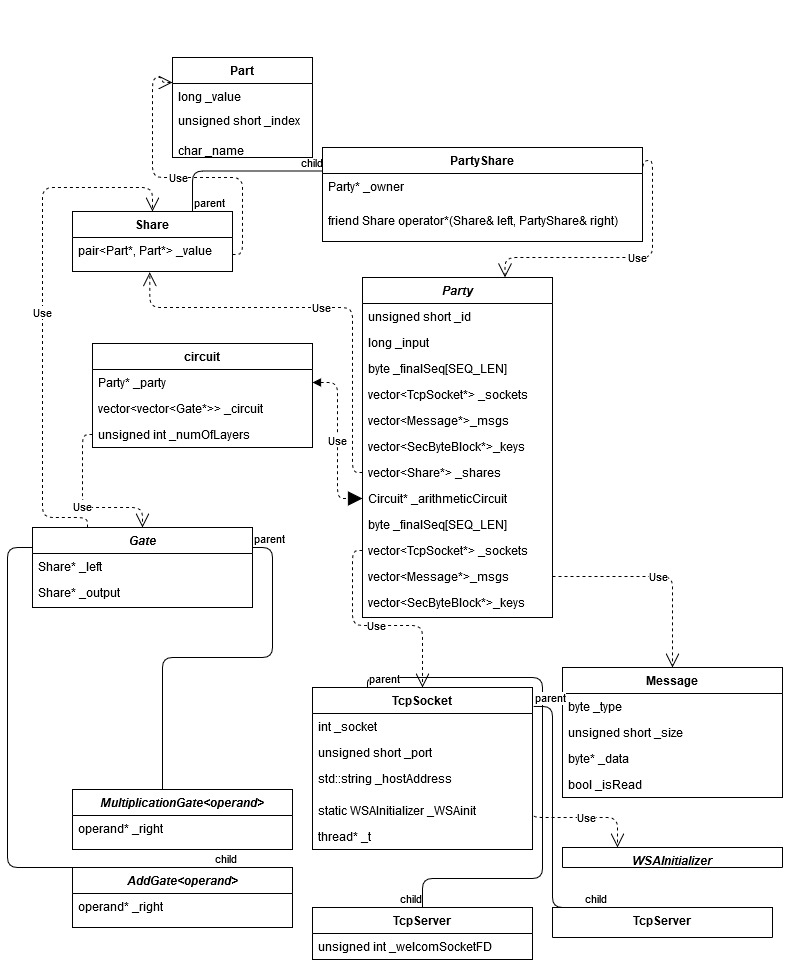
\includegraphics[width=13cm, height=13cm]{"../Figures/classes.jpeg"}}%
  \caption{Classes}
  \label{fig:Classes}
\end{figure}

This diagram represent the relations between the classes, the classes described below.
\pagebreak
\subsection{Party:}
This class represents a participant in the protocol. All the communication between the parties is performed via this class. To execute the protocol, the following functions should be called: connectToAllParties, fInput, calcCircuit and reconstruct in the specified order.
After the main thread performs the connectToAllParties function the vector sockets contain all the sockets to the other parties through which the future messages of the protocol will be sent.
Moreover, the class contains a vector of shares, one share per input to the circuit. After the execution of fInput this vector holds the shares this party suppose to have as discussed in the paper.
Additionally, the party has a pointer to the arithmetic circuit which needs to be calculated.
Finally, the party holds a vector of Messages of unread messages this party received. A message marked as read if the main thread got the message.
\hfill\break

\textbf{Variables:}
\begin{itemize}
	\item short id: Unique identifier, lowest ip receive id = 1. 
	\item long input: secret input.
	\item byte finalSeq: Mutual counter for all participents.
	\item vector$<$TcpSocket*$>$sockets: Socket for all TCP connection with other parties.
	\item vector$<$Message*$>$msgs: Vector which contains all recieved messages.
	\item vector$<$SecByteBlock*$>$keys: Vector which contains all the keys required for generating random numbers.
	\item vector $<$Share*$>$ shares: Vector which contains each party's share.index of vector is the id of input's party.
	\item Circuit* arithmeticCircuit: The function which needs to be computed.
\end{itemize}
\textbf{Functions:}
\begin{itemize}
	\item sendTo: Send message to party[id].
	\item readFrom: Read message from party number id. this is a blocking function.
	\item connectToAllParties: This function is responsible o setting connectivity between al parties. Each party $p_i$ has two TCP connections to party $p_{(i+1)}$ and party $p_{(i-1)}$ 
	\item broadcast: Send message to all parties
	\item getShare: Getter by index for the shares held by this party.
	\item setShare: Setter by index for the shares held by this party.
	\item getID: Getter for this party ID.
	\item calcSeq: Calculate the joint seq. Initiates at the begining of the protocol.
	\item calcCircuit: Calculate the output of all the gates in the circuit.
	\item fRand: fRand functuality as described in the paper.
	\item reconstruct: Receives all the Parts of a given share.
\end{itemize}


\subsection{TcpSocket:}
This class represent a generic TCP socket. It has a static member WSAInitializer to allow communication via sockets. This class also contains a thread which waits for new messages to come from this socket. Each party functions as both a server and a client. It is a server for Party $p_{i-1}$ and a client for Party $p_{i+1}$ to keep it symmetric. 
\hfill\break

\textbf{Variables:}
\begin{itemize}
	\item int socket: FD of the socket.
	\item int port: Port number
	\item string hostAddress: IP address of the host.
	\item WSAInitializer WSAinit: All processes that call Winsock functions must initialize the use of the Windows Sockets DLL before making other Winsock functions calls. This also makes certain that Winsock is supported on the system.
	\item thread t: Thread for receiving messages.
\end{itemize}
\textbf{Functions:}
\begin{itemize}
	\item id : Return the socket descriptor.
	\item port: Return the socket port number.
	\item writeBuffer: Write a buffer over the socket connection.  Returns the number of bytes written or -1 if an error occurs.
	
	\item readBuffer: Read an input buffer, up to length bufferSize.  Returns the number of bytes read or -1 if an error occurs.
	
	\item isValid: Returns true if the socket descriptor is valid.
	\item socketFd: Return id of the socket if valid.
	\item close: Close all connections.
	\item messagesHandler: Receive all messages coming via socket.
\end{itemize}


\subsection{TcpClient:}
This class represent a TCP client which inherits from TcpSocket class. This class initiate a TCP connection with the party $p_{i+1}$.\hfill\break\hfill\break

\textbf{Variables:}\hfill\break
  \begin{itemize}
	\item No extra variables.
\end{itemize} \hfill\break
\textbf{Functions:}
\begin{itemize}
	\item connect: Connect to some server.
\end{itemize}
\subsection{TcpServer:}
This class represent a TCP server which inherits from TcpSocket class. This class waits the party with id-1 to initiate a TCP connection with it.\hfill\break

\textbf{Variables:}
\begin{itemize}
\item welcomSocketFD: Welcome socket fd.
\end{itemize}
\textbf{Functions:}
\begin{itemize}
	\item serve: Bind + Listen + Accept. Throws an exception in case of failure.
	
	\item accept: Accept a new connection
\end{itemize}

\subsection{Part:}
This class represent the first and second parts in each share. It has value, index, and a single character to indicate what expression this parts construct together.
The addition of all three parts would give us the value of what they represent.\hfill\break

\textbf{Variables:}
\begin{itemize}
\item value: The value of the part.
\item index: The index of the part.
\item name: The name of the part
\end{itemize}

\textbf{Functions:}
\begin{itemize}
\item Geters \& Setters.
\item toString: Prints the share.
\item operator$=$: updates the Part value, index and name if needed.
\end{itemize}
\subsection{Share:}
This class represent a share as defined in the paper. The share object is implemented using an attribute of type pair. The first part and the second are pointers to Parts of the share.\hfill\break

\textbf{Variables:}
\begin{itemize}
\item pair$<$Part*, Part*$>$ value: Share as described on the article.
\end{itemize}
\textbf{Functions:}
\begin{itemize}
	\item getFirst \& getSecond: Return the First/Second part of the share.
	\item getOwnerId: Return the ID of the owner of the share.
	\item isAddable: Checks if two Shares can be added.
	\item operator=: Updates the Share.
	\item operator+(with Share): implements the addition of two Shares.
	\item operator+(with constant): implements the addition of Share and constant.
	\item operator[]: Return A part of the Share.
	\item operator*: implements the multiplication of two Share with constant.
	\item toString: Prints the Share.
\end{itemize}
\subsection{PartyShare:}
This class inherits from Share class. The purpose of this class is to allow communication during the calculation of the multiplication gate. In addition to the original share information PartyShare also contains a pointer to the party which possess the share, to perform communication.\hfill\break

\textbf{Variables:}
\begin{itemize}
\item  Party* owner: the owner of the Share.
\end{itemize}
\textbf{Functions:}
\begin{itemize}
	\item correlatedRandomness: calculate correlated randomness as described in paper.
	\item getParty: return the owner.
	\item operator*: implimentation of the multplication of two shares as described in the paper.
\end{itemize}
\subsection{WSAInitializer:}
Initialize some DLL files so the windows operation system will allow the program to open and use the sockets. This object should be constructed only once.\hfill\break

\textbf{Functions:}
\begin{itemize}
	\item constructor: the initialization is made in the constructor.
\end{itemize}
\subsection{Massages:}
This class describe an massage.\hfill\break

\textbf{Variables:}
\begin{itemize}
\item type: An identifier to ID each type of message.
\item size: The size of the accusal message without header(type+size).
\item data: Array of length size + 1 for null character.
\item isRead: flag to inidicate if the message was read.

\end{itemize}
\textbf{Functions:}
\begin{itemize}
	\item Getters \& Setters.
\end{itemize}
\subsection{Helper:}
Some functions.\hfill\break

\textbf{Variables:}
\begin{itemize}
\item No variables.
\end{itemize}
\textbf{Functions:}
\begin{itemize}
	\item IPCompare: Return true if first is greater than second.
	\item encryptAES:Perform an AES encryption.
\end{itemize}
\subsection{Gate:}
The class represent a gate in the circuit to calculate. Gate is abstract class, base class for AddGate \& multiplicationGate. Each gate has two inputs wire and output wire, the left wire is always an share but right wire can be share or constant. The Gate class has only the left wire(right wire is in the Add/Multiplication gate.) \hfill\break

\textbf{Variables:}
\begin{itemize}
	\item Share* left: left input wire.
	\item Share* output: output wire.
\end{itemize}
\textbf{Functions:}
\begin{itemize}

	\item Getters \& Setter.
	\item calculateOutput: Pure virtual function, implemented in Addition/Multipication classes. Calculate the output of this Gate(Addition/Multipication).

\end{itemize}
\subsection{AdditionGate:}
A template class inherits from the abstract class Gate. This class represent an addition gate. It has an attribute that represent the right input to the gate. The type of this attribute can be a constant of type long or a share type.\hfill\break

\textbf{Variables:}
\begin{itemize}
\item operand* right: The right wire of an gate, operand is an template variable, can be constant or Share.
\end{itemize}
\textbf{Functions:}
\begin{itemize}
	\item calculateOutput: overide the base class calculateOutput function.
\end{itemize}
\subsection{MultiplicationGate:}
A template class inherits from the abstract class Gate. This class represent a multiplication gate. It has an attribute that represent the right input to the gate. The type of this attribute can be a constant of type long or a share type.\hfill\break

\textbf{Variables:}
\begin{itemize}
\item operand* right: The right wire of an gate, operand is an template variable, can be constant or Share.
\end{itemize}
\textbf{Functions:}
\begin{itemize}
	\item calculateOutput: overide the base class calculateOutput function.
\end{itemize}
\subsection{Circuit:}
This class represent the arithmetic circuit all 3 parties calculating together. The circuit contains layers of aggregation toward the output of the circuits. Each layer contains a pointer to an additionGate or a MultipicationGate which inherits from the abstract class Gate.
The circuit class also contains a pointer to the party. The reason for that is to forward this pointer to the PartyShare class at its construction. The circuit class creates PartyShare if the circuit contains a multiplication gate.
\hfill\break

\textbf{Variables:}
\begin{itemize}
\item Party* party: in order to perform communication rounds in multipication gates an access to Party is required.
\item vector$<$vector$<$Gate*$>>$ circuit: Layers of gates, first index is the layer index and the second index is the gate's index within each layer.
\item numOfLayers: Number of layers.
\item vector$<$int$>$ gatesPerLayer: Number of gates in each layer of the circuits.

\end{itemize}
\textbf{Functions:}
\begin{itemize}
	\item calculateOutput: Computes the outout of each gate.
	\item getOutput: Get the result of the circuit.
\end{itemize}
\subsection{Library used}
\begin{itemize}
	\item \textbf{WinSock2}: Winsock provides the programming interface for applications to communicate using popular network protocols such as TCP \& UDP and provide a large set of network functions 
	\item \textbf{OpenSSL}: its an open source library for applications that secure communications over computer networks against eavesdropping or need to identify the party at the other end. downloaded from $https://www.openssl.org/$\break \textbf{We decided to use Crypto++ instead.}
	
	\item\textbf{Crypto++}: Also known as CryptoPP, libcrypto++ is a free and open-source C++ class library of cryptographic algorithms and schemes. can be downloaded from $https://www.cryptopp.com/\#download$, we used the latest version, Crypto++ 8.2.0.
\end{itemize}
\pagebreak
\section{Run the code:}
\subsection{Install Crypto++:}
In order to run or compile the code in visual studio Crypto++ library is required. TO install the library follow the next steps (or Google it: "Crypto++ visual studio"):
\begin{enumerate}
	\item Download Crypto++ 8.2.0 (if there is newest version, they should work) from : $https://www.cryptopp.com/\#download$
	\item As soon as your download will be finished, extract the content of the zip in a folder of your choice(We recommend in $C:/Program Files/Crypto++$).
	\item Navigate to your Crypto++ source folder and look for a file named cryptest.sln. Right click on it $->$ open with $->$ Visual Studio 2019

\item Right click on cryptlib $->$ properties $->$ Configuration properties $->$ Code Generation $->$ Runtime Library $->$ Change to Multi-threaded Debug (MTd) $->$ Close the menu.
\item Click the Build menu $->$ Batch Build $->$ Select cryptlib Debug x64 and cryptlib Release x64 $->$ Build.
\item Open Final-Project with visual Studio 2019. Then go to the Project properties by right clicking your project.
\item properties $->$ Configuration properties $->$  C/C++ $->$ Additional Include Directories $->$ Select the Crypto++ folder (C:/Program Files/Crypto++)
\item properties $->$ Configuration properties $->$ Linker $->$ Input $->$ Additional Dependency $->$ Enter the cryptlib.lib path(cryptlib.lib is in the folder Crypto++, C:/Program Files/Crypto++/x64/cryptlib select release or debug folder according the running configuration)
\end{enumerate}
\subsection{Enter Parameters:}
The application need to receive all the participants IPs.
The first parameter is the Party IP, the two other IPs its the other Parties IP, for example my ip is 192.168.0.2 and other PCs IPs is : 192.168.0.3 and 192.168.0.4, if running in debug mode:
\begin{itemize}
\item Click on Debug menu $->$ Final-Project Debug Properties $->$Configuration properties $->$ Debugging $->$ Command  Arguments $->$  192.168.0.2 192.168.0.3 192.168.0.4 OR 192.168.0.2 192.168.0.4 192.168.0.3
\end{itemize}
Or if running in release mode :
\begin{itemize}
\item Open CMD $->$ Navigate to Project executable $->$ final-Project 192.168.0.2 192.168.0.3 192.168.0.4 OR final-Project 192.168.0.2 192.168.0.4 192.168.0.3
\end{itemize}
\pagebreak
\section{Future work}

\begin{enumerate}
	\item Name - The name attribute of Part class was created to indicate what variable this part constructs. That is, every party has 3 shares (each one consists of 2 Parts) in total at the beginning of the arithmetic circuit. E.g. suppose the shares to the circuit are $||x||$, $||y||$ and $||z||$ then the names would be 'x', 'y' and 'z' respectively. The problem is that the output of an addition gate (which its inputs are: $||x||$ and $||y||$) is a share with no name instead of 'x+y' as expected.
	\item Mutex – The current form of synchronization of the threads is performed using Party class attributes. This needs to be changed to mutexes.
	\item Circuit – At this point the circuit is randomly calculated synchronically using a common seed. It is required to add another constructor to Circuit class which build a specific circuit according to some parameters sent to the constructor.
	\item $F_{vrfy}$ - In order to finish the project it necessary to implement $F_{vrfy}$, we planed to implement it but we faced few issues during the second semester(issues such COVID-19). To compare the linear algorithm to previous work, its require to implement the "slow" algorithm also. 
\end{enumerate}
\pagebreak
\section{Timeline}


\subsection{Milestones}
Milestone planning is one of the most important aspects of project planning, because project milestones are the most visible indicators of project progress. Milestones typically mark critical decision points, the completion of major project tasks and the ends of various project phases. 
\hfill\break
As seen in Millstones table - table: \ref{tab:Millstones} we changed the subject of our project. First research was on OT extension protocol, then on homomorphic secret sharing and finally fully secure 3MPC. we chose to change our project subject because OT extension and hommomorfic secret sharing are more research than coding. This decision caused delay in progress but increased our motivation.

\begin{table}
\caption{Millstones}
\begin{center}
\begin{tabular}{|c|p{4 cm}|c|c|p{3.5 cm}|}
	\hline
	 & Task name & Meet time &Work days& Outcome \\	
	\hline 
	1&Research OT extension& 20/10/19 & 14 & knowlage \\ 
	\hline
	2&Research Hommomorphic secret sharing& 05/11/19 & 14 & knowlage \\
	\hline
	3&Research fully secure 3MPC& 10/12/19 & 14 & knowlage \\
	\hline
	4&Prework report& 29/12/19 & 5 &Prework for the progress report \\
	\hline
	5&Code design for Connectivity & 10/1/20 & 3 & Code design\\
	\hline
	6&Implementing Connectivity& 25/1/20 & 5 & Connectivity between 3 PC's\\
	\hline
	7&Progress report & 26/1/20 & 7 & Progress and research report \\
	\hline
	8&Code design for secret sharing  & 3/2/20 & 2 & Code design\\
	\hline
	9&Implementing secret sharing  & 15/2/20 & 5 &Code for sharing the secret input \\
	\hline
	10&Code design for the logic circuit  & 25/2/10 & 2 & Code design\\
	\hline
	11&Implementing the logic circuit  & 5/3/20 & 7 & working Boolean circuit function calculation\\
	\hline
	12&Code design for verify function  & 15/3/20 & 3 & Design for the verify function\\	
	\hline
	13&Implementing verify function  & 1/4/20 & 14 & complete all part of the project\\	
	\hline
	14&Testing and benchmark & 22/4/20 & 7 & Fixing bugs and getting results\\
	\hline
	15&Poster & 06/20 & 14 & Poster for presentation\\
	\hline
	16&Presentation & 06/20 & 14 &Presenting the project\\
	\hline
	17&Final submission & 08/20 & 14 & Submiting the project\\
	\hline
\end{tabular}
\end{center}
\label{tab:Millstones}
\end{table}

\pagebreak
\subsection{Gant}

\begin{figure}[h!]
	\centering
	\includegraphics[scale=0.8]{"../Figures/gant_new"}
	\caption{Gant}
	\label{fig:gantfig1}
\end{figure}


\pagebreak
\section{Bibliography}
\begin{thebibliography}{9}
	
	\bibitem{main}
	Dan Boneh and Elette Boyle and Henry Corrigan-Gibbs and Niv Gilboa and Yuval Ishai
	\textit{ "Practical Fully Secure Three-Party Computation via Sublinear Distributed Zero-Knowledge Proofs."}
	In Proceedings of the 2019 ACM SIGSAC Conference on Computer and Communications Security, pp. 869-886. ACM, 2019.
	
	\bibitem{main_based}
	Boyle, Elette, Niv Gilboa, Yuval Ishai, and Ariel Nof
	\textit{ "Zero-Knowledge Proofs on Secret-Shared Data via Fully Linear PCPs."}
	Cryptology ePrint Archive, Report 2019/188.

	\bibitem{f_input}
	Koji Chida and Daniel Genkin and Koki Hamada and Dai Ikarashi and Ryo Kikuchi and Yehuda Lindell and Ariel Nof
	\textit{ "Fast Large-Scale Honest-Majority MPC for Malicious Adversaries"}
	Cryptology ePrint Archive, Report 2018/570.
	
	\bibitem{sync_async}
	Dani, Varsha, Valerie King, Mahnush Movahedi, Jared Saia, and Mahdi Zamani
	\textit{ "Secure multi-party computation in large networks"}
	Distributed Computing 30, no. 3 (2017): 193-229.
	
	\bibitem{OT}
	Elette Boyle and Geoffroy Couteau and Niv Gilboa and Yuval Ishai and Lisa Kohl and Peter Rindal and Peter Scholl
	\textit{ "Efficient Two-Round OT Extension and Silent Non-Interactive Secure Computation"}
	Cryptology ePrint Archive, Report 2019/1159
	
	\bibitem{homomrphic_secret_sharing}
	Elette Boyle and Geoffroy Couteau and Niv Gilboa and Yuval Ishai and Michele Orrù
	\textit{ "Homomorphic Secret Sharing: Optimizations and Applicationsks"}
	Cryptology ePrint Archive, Report 2018/419.
	
	\bibitem{replicated_secret_sharing}
	Furukawa, Jun and Lindell, Yehuda
	\textit{ "Two-Thirds Honest-Majority MPC for Malicious Adversaries at Almost the Cost of Semi-Honest"}
	Proceedings of the 2019 ACM SIGSAC Conference on Computer and Communications Security.
	
	\bibitem{temp0}
	Eerikson, Hendrik, Claudio Orlandi, Pille Pullonen, Joonas Puura and Mark Simkin.
	\textit{ "Use your Brain! Arithmetic 3PC For Any Modulus with Active Security"}
	IACR Cryptology ePrint Archive 2019 (2019): 164.

	\bibitem{temp1}
	Furukawa, Jun and Lindell, Yehuda and Nof, Ariel and Weinstein, Or.
	\textit{ "High-Throughput Secure Three-Party Computation for Malicious Adversaries and an Honest Majority"}
	Advances in Cryptology – EUROCRYPT 2017.

	\bibitem{MPC_applications}
	 David Evans, Vladimir Kolesnikov and Mike Rosulek, A Pragmatic 	
	\textit{ "Introduction to Secure Multi-Party Computation.."}
	 NOW Publishers, 2018
	
\end{thebibliography}
\pagebreak


\end{document}
